%===================================================================================
% JORNADA CIENTÍFICA ESTUDIANTIL - MATCOM, UH
%===================================================================================
% Esta plantilla ha sido diseñada para ser usada en los artículos de la
% Jornada Científica Estudiantil de MatCom.
%
% Por favor, siga las instrucciones de esta plantilla y rellene en las secciones
% correspondientes.
%
% NOTA: Necesitará el archivo 'jcematcom.sty' en la misma carpeta donde esté este
%       archivo para poder utilizar esta plantila.
%===================================================================================



%===================================================================================
% PREÁMBULO
%-----------------------------------------------------------------------------------
\documentclass[a4paper,10pt,twocolumn]{article}

%===================================================================================
% Paquetes
%-----------------------------------------------------------------------------------
\usepackage{amsmath}
\usepackage{amsfonts}
\usepackage{amssymb}
\usepackage{jcematcom}
\usepackage[utf8]{inputenc}
\usepackage{listings}
\usepackage[pdftex]{hyperref}
\usepackage{caption}
\usepackage{subcaption}
\usepackage{graphicx}
\usepackage{float}
\usepackage{algorithm}
\usepackage{algpseudocode}
%-----------------------------------------------------------------------------------
% Configuración
%-----------------------------------------------------------------------------------
\hypersetup{colorlinks,%
	    citecolor=black,%
	    filecolor=black,%
	    linkcolor=black,%
	    urlcolor=blue}

%===================================================================================



%===================================================================================
% Presentacion
%-----------------------------------------------------------------------------------
% Título
%-----------------------------------------------------------------------------------
\title{Detectando Interacciones en Coros de Colines (\textit{Eleutherodactylus eileenae}). Un enfoque desde el Modelo de Ising.}

%-----------------------------------------------------------------------------------
% Autores
%-----------------------------------------------------------------------------------
\author{\\
\name Daniel Machado Pérez \email \href{mailto:daniel.machado.0206@gmail.com}{daniel.machado.0206@gmail.com}
	\\ \addr Grupo C411}

%-----------------------------------------------------------------------------------
% Tutores
%-----------------------------------------------------------------------------------
\tutors{\\
Dr. Roberto Mulet, \emph{Facultad de Física, UH} \\
Dr. Milton García, \emph{Centro de Sistemas Complejos, UH}\\
Dr. Roberto Alonso, \emph{Facultad de Biología, UH}}

%-----------------------------------------------------------------------------------
% Headings
%-----------------------------------------------------------------------------------
\jcematcomheading{\the\year}{1-\pageref{end}}{D. Machado}

%-----------------------------------------------------------------------------------
\ShortHeadings{Detectando Interacciones en Coros de Colines}{Daniel Machado Pérez}
%===================================================================================



%===================================================================================
% DOCUMENTO
%-----------------------------------------------------------------------------------
\begin{document}

%-----------------------------------------------------------------------------------
% NO BORRAR ESTA LINEA!
%-----------------------------------------------------------------------------------
\twocolumn[
%-----------------------------------------------------------------------------------

\maketitle

%===================================================================================
% Resumen y Abstract
%-----------------------------------------------------------------------------------
\selectlanguage{spanish} % Para producir el documento en Español

%-----------------------------------------------------------------------------------
% Resumen en Español
%-----------------------------------------------------------------------------------
\begin{abstract}

	Este estudio presenta un nuevo enfoque para analizar 
	las interacciones en coros de \emph{Eleutherodactylus 
	eileenae} (Colín) a partir de grabaciones de campo. 
	Se parte de la metodología desarrollada en trabajos previos, 
	en la que se identificaron secuencias de cantos mediante 
	técnicas de extracción de mel-espectrogramas, detección de 
	picos de energía y sincronización de señales a través de 
	correlación cruzada. En el presente trabajo se incorporan 
	mejoras en el preprocesamiento de la información, como la 
	eliminación de ruido basada en el percentil 99.9 y un 
	algoritmo automático de sincronización, que permiten 
	obtener datasets de mayor calidad. Posteriormente, 
	se modela el sistema acústico mediante el Modelo de Ising, 
	permitiendo la inferencia exacta de los parámetros de 
	interacción (\( J_{ij} \)) a partir de 
	la enumeración total de las \(2^9 = 512\) configuraciones 
	posibles. Los resultados obtenidos revelan la presencia de 
	interacciones fuertes y persistentes, lo que sugiere una 
	organización estructural en el comportamiento colectivo del 
	coro. 


\end{abstract}

%-----------------------------------------------------------------------------------
% English Abstract
%-----------------------------------------------------------------------------------
\vspace{0.5cm}

\begin{enabstract}

	This study presents a novel approach to analyze interactions 
	in choruses of \emph{Eleutherodactylus eileenae} (Colín) 
	using field recordings. Building upon a previously 
	developed methodology—which identified call sequences 
	using mel-spectrogram extraction, energy peak detection, 
	and cross-correlation-based synchronization—the present 
	work incorporates improvements in data preprocessing, 
	such as noise elimination based on the 99.9th percentile 
	and an automatic synchronization algorithm, to obtain 
	higher quality datasets. Subsequently, the acoustic 
	system is modeled using the Ising model, allowing for 
	the exact inference of interaction parameters 
	(\( J_{ij} \)) by enumerating all \(2^9 = 512\) possible 
	configurations. The obtained results reveal the presence of 
	strong and persistent interactions, suggesting a structured 
	organization in the collective behavior of the chorus.

\end{enabstract}

%-----------------------------------------------------------------------------------
% Palabras clave
%-----------------------------------------------------------------------------------
\begin{keywords}
	Colín, Modelo de Ising, Inferencia Estadística, Descenso por Gradiente, Procesamiento de Señales.
\end{keywords}

%-----------------------------------------------------------------------------------
% Temas
%-----------------------------------------------------------------------------------
\begin{topics}
	Inteligencia Artificial, Matemática Aplicada.
\end{topics}


%-----------------------------------------------------------------------------------
% NO BORRAR ESTAS LINEAS!
%-----------------------------------------------------------------------------------
\vspace{1cm}
]
%-----------------------------------------------------------------------------------


%===================================================================================

%===================================================================================
% Introducción
%-----------------------------------------------------------------------------------
\section{Introducción}\label{sec:intro}
%-----------------------------------------------------------------------------------
La rana \emph{Eleutherodactylus eileenae} (Colín, Figura \ref{fig:elena}) es una 
especie de la familia \emph{Eleutherodactylidae} endémica 
de Cuba, ampliamente distribuida en las zonas occidental y 
central de la isla \cite{alonso2001patrones}. Su canto de 
apareamiento es característico, compuesto por dos señales 
distintivas: una de frecuencia baja, denominada \emph{CO}, y 
otra de frecuencia alta, denominada \emph{LIN}. Estas emisiones 
se organizan en secuencias repetitivas que, al conformar un 
coro, sugieren la existencia de patrones de sincronización y 
de regulación de frecuencia en respuesta a las interacciones 
acústicas entre individuos.

\begin{figure}[htbp]
    \centering
    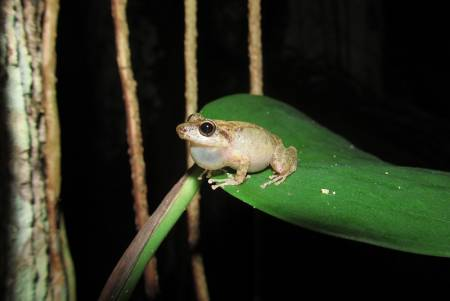
\includegraphics[width=\columnwidth]{assets/elena.jpg}
    \caption{Ejemplar de \emph{Eleutherodactylus eileenae}.}
    \label{fig:elena}
\end{figure}

En investigaciones previas se desarrolló el estudio titulado 
\href{https://github.com/DanielMPMatCom/Identifying-Colines.-JCE-MatCom.git}{\emph{Identificando Colines (Eleutherodactylus eileenae) a 
partir de audios desordenados}}, en el que se diseñó una 
metodología computacional para identificar las secuencias 
probables de cantos a partir de grabaciones de campo realizadas 
con nueve micrófonos durante 3 días, a partir de las 18:00 hasta 
las 06:00 horas del día siguiente. Para visualizar la 
distribución geográfica de los 
dispositivos véase la Figura \ref{fig:mics}.
Cada micrófono, colocado 
estratégicamente en el entorno natural, registró 58 minutos 
consecutivos, seguidos de un breve lapso de inactividad, 
durante los períodos de mayor actividad (desde el atardecer 
hasta el amanecer). Los métodos implementados incluyeron la 
utilización de mel-espectrogramas \cite{zhang2021acoustic} (Figura \ref{fig:mel}), extracción de picos de 
energía, y técnicas de sincronización basadas en correlación 
cruzada \cite{costa2021comparing}, permitiendo así discriminar, a partir de la mezcla de 
señales, el canto emitido por el individuo más próximo a cada 
micrófono. 


\begin{figure}[htbp]
    \centering
    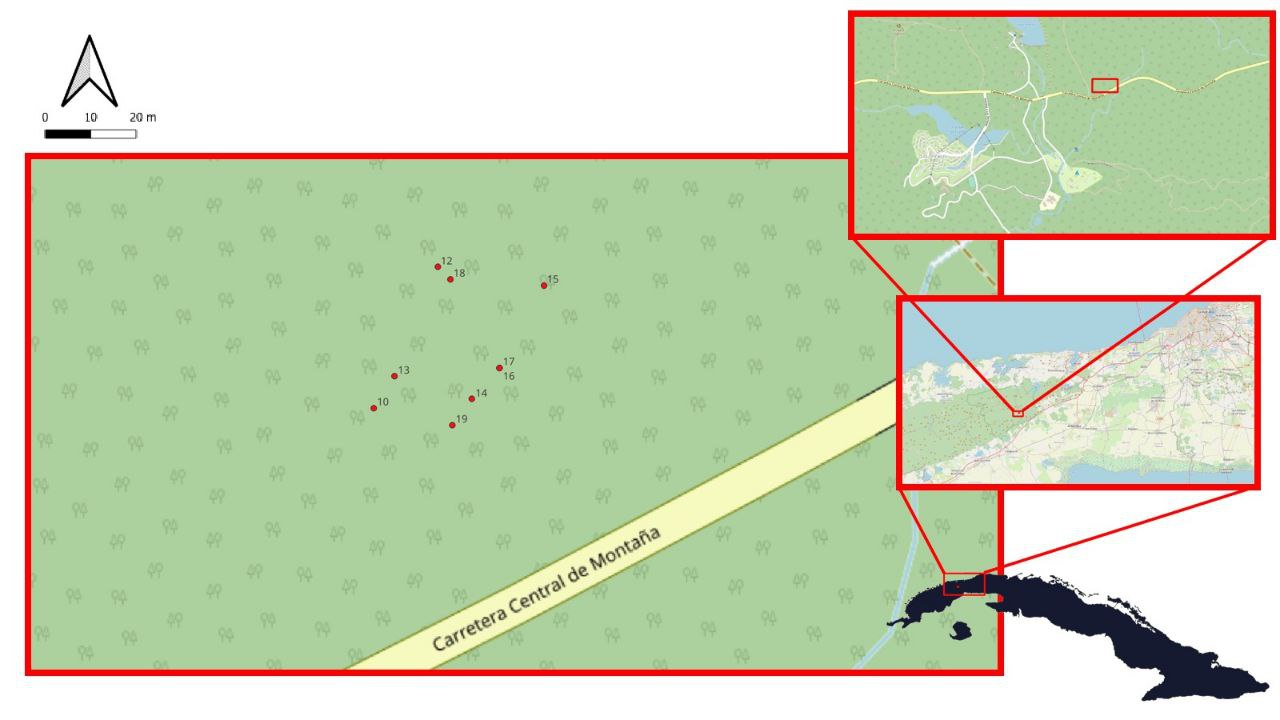
\includegraphics[width=\columnwidth]{assets/mic_map.jpg}
    \caption{Distribución Geográfica de los Micrófonos.}
    \label{fig:mics}
\end{figure}

\begin{figure}[htbp]
    \centering
    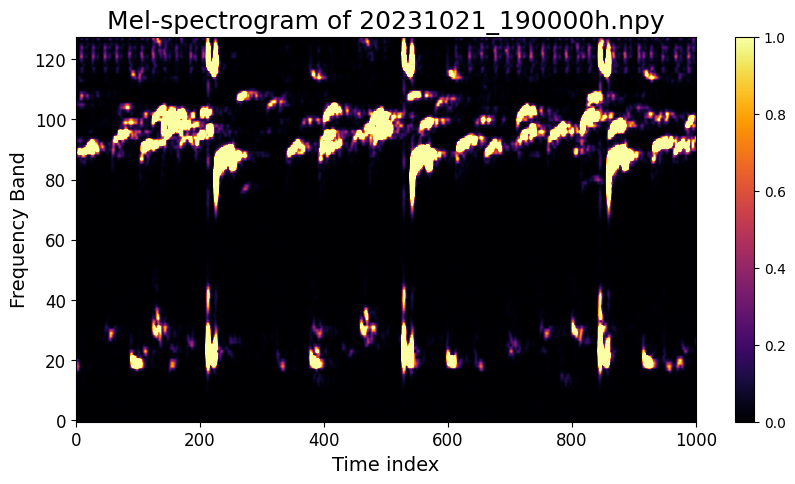
\includegraphics[width=\columnwidth]{assets/mel-spectrogram.png}
    \caption{Ejemplo de mel-espectrograma de un fragmento de audio del conjunto de datos.}
    \label{fig:mel}
\end{figure}

\subsection{Actualizaciones y mejoras}

Como mejoras respecto al estudio anterior, se ha incorporado un nuevo esquema de eliminación de ruido, que utiliza el percentil 99.9 para filtrar los valores atípicos y descartar contribuciones espurias en las señales. Además, se implementó un algoritmo de sincronización automático, basado en el análisis detallado de las energías temporales, que optimiza la alineación de los audios de las diversas fuentes. Estos avances permiten obtener conjuntos de datos de mayor calidad y consistencia, proporcionando una base robusta para la exploración de la dinámica y la causalidad en las interacciones del coro.

Como resultado del trabajo mencionado se logró obtener un \textit{dataset}
limpio, donde se guarda por separado la información de los cantos de
Colines, de tal forma que es posible estudiar coros como el que se observa 
en la Figura \ref{fig:seq}.

\begin{figure}[htbp]
    \centering
    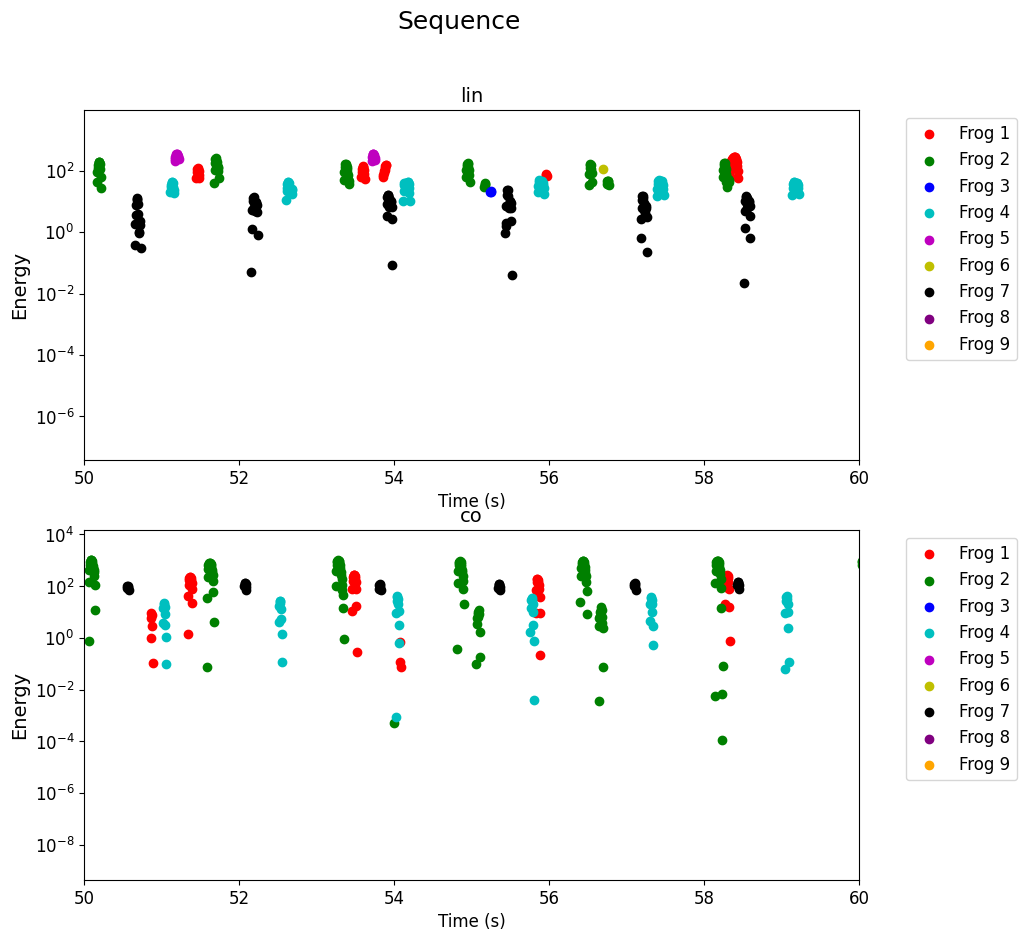
\includegraphics[width=\columnwidth]{assets/sequence.png}
    \caption{Gráfica del comportamiento de la Energía en el Tiempo, donde cada color representa un Colín distinto.}
    \label{fig:seq}
\end{figure}

\subsection{Nuevos retos}

La presente investigación se enfoca en ampliar el análisis 
previo, abordando la tarea de modelar y cuantificar las 
interacciones entre los individuos mediante un 
\emph{Modelo de Ising} \cite{chau2017inverse}. 

El Modelo de Ising es un marco matemático fundamental en la física estadística, originalmente concebido para describir la interacción de espines en sistemas magnéticos. En este modelo, cada componente se representa mediante una variable binaria \( \sigma_i \in \{-1,+1\} \), que asume uno de dos estados posibles. Las interacciones entre estos espines se cuantifican a través de parámetros \( J_{ij} \), y además se incluye un campo externo \( h_i \) que influye en el comportamiento individual. Gracias a su formulación, el Modelo de Ising permite estudiar fenómenos cooperativos y transiciones de fase en sistemas complejos, siendo aplicable no solo en magnetismo, sino también en diversas áreas como la biología, la informática y la inferencia estadística.


En este marco, cada Colín se asocia a un espín \( \sigma_i \in \{-1, +1\} \), donde \( +1 \) indica la emisión de canto y \(-1\) su ausencia. La distribución de probabilidad del sistema se modela a partir de la distribución de Boltzmann:

\[
P(\boldsymbol{\sigma}) = \frac{1}{Z} \exp\Biggl( \sum_{i<j} J_{ij}\, \sigma_i \sigma_j + \sum_{i} h_i\, \sigma_i \Biggr),
\]

donde \( Z \) es la función de partición, y los parámetros \( J_{ij} \) y \( h_i \) representan, respectivamente, las intensidades de las interacciones entre pares de individuos y los sesgos o influencias individuales. Gracias al reducido número de espines (\( N = 9 \)), es posible calcular de manera exacta \( Z \) mediante la enumeración de las \( 2^9 \) configuraciones, lo que permite llevar a cabo una inferencia precisa de los parámetros a través de un algoritmo de descenso por gradiente. Este enfoque no solo facilita la identificación de interacciones significativas —por ejemplo, determinando aquellas que se mantienen fuertes y persistentes a lo largo del tiempo— sino que además sienta las bases para el análisis causal y la comprensión de la estructura subyacente del comportamiento colectivo del coro.

Con el modelo matemático así definido, el presente artículo desarrolla la inferencia de los parámetros del sistema, explorando las relaciones de causalidad y correlación entre los individuos y proponiendo un nuevo enfoque en el análisis de interacciones acústicas basado en herramientas de la física estadística.

%===================================================================================



%===================================================================================
% Desarrollo
%-----------------------------------------------------------------------------------
\section{Desarrollo}\label{sec:dev}
%-----------------------------------------------------------------------------------
  
Con el objetivo de estudiar las posibles dependencias e 
influencias mutuas entre los individuos del coro, 
se plantea modelar su comportamiento mediante un sistema 
estadístico en equilibrio. Aunque las vocalizaciones de los 
Colines no constituyen en sí un proceso estrictamente 
estacionario, se considera una aproximación inicial útil 
suponer que el sistema se encuentra en equilibrio termodinámico. 
Esta hipótesis permite el uso de herramientas de la física 
estadística y proporciona un marco riguroso para analizar las 
correlaciones observadas.

La idea central consiste en inferir la estructura de 
interacciones entre los individuos del sistema, es decir, 
determinar qué tan probable es que un Colín cante dado el 
estado acústico de los demás. Para modelar estas relaciones 
se utiliza el conocido \textit{Modelo de Ising}, el cual ha 
sido ampliamente empleado en física, biología y ciencias de 
la computación para describir sistemas de componentes binarios 
que interactúan sobre una red.

En el modelo propuesto, cada Colín se asocia a un 
espín \( \sigma_i \in \{-1, +1\} \), donde 
\( \sigma_i = +1 \) indica que el individuo está vocalizando en 
un instante dado, y \( \sigma_i = -1 \) que no lo está. 
El conjunto de estados 
\( \boldsymbol{\sigma} = (\sigma_1, \dots, \sigma_N) \), 
donde \( N = 9 \), representa una configuración global del 
sistema. A partir de esta representación binaria, el modelo 
establece una distribución de probabilidad sobre todos los 
posibles estados, dada por la distribución de Boltzmann:

\[
P(\boldsymbol{\sigma}) = \frac{1}{Z} \exp\left( \sum_{i<j} J_{ij} \sigma_i \sigma_j + \sum_{i} h_i \sigma_i \right),
\]

donde \( J_{ij} \) representa la fuerza de interacción entre 
los individuos \( i \) y \( j \), \( h_i \) es un campo 
externo (o sesgo individual), y \( Z \) es la función de 
partición que garantiza la normalización:

\[
Z = \sum_{\boldsymbol{\sigma}} \exp\left( \sum_{i<j} J_{ij} \sigma_i \sigma_j + \sum_i h_i \sigma_i \right).
\]

Este modelo puede entenderse también como una red no dirigida 
en la que cada nodo (espín) se conecta a los demás mediante 
pesos \( J_{ij} \). En analogía con las redes neuronales o los 
modelos gráficos probabilísticos, las conexiones codifican 
correlaciones estadísticas que se busca estimar a partir de 
datos observados.

Dado un conjunto de configuraciones 
\(\{\boldsymbol{\sigma}^{(1)}, \dots, \boldsymbol{\sigma}^{(M)}\}\) 
obtenidas del sistema real (en este caso, instantes discretos 
de la secuencia de cantos), el objetivo es encontrar los 
parámetros \( J_{ij} \) y \( h_i \) que maximizan la 
verosimilitud del modelo \cite{zeng2013maximum}. Esto equivale a resolver el 
siguiente problema de optimización:

\[
\mathcal{L}(J, h) = \sum_{m=1}^{M} \log P(\boldsymbol{\sigma}^{(m)}),
\]

cuyo gradiente con respecto a \( J_{ij} \) se expresa como:

\[
\frac{\partial \mathcal{L}}{\partial J_{ij}} = \langle \sigma_i \sigma_j \rangle_{\text{datos}} - \langle \sigma_i \sigma_j \rangle_{\text{modelo}},
\]

donde el primer término es la correlación empírica entre los 
espines \( i \) y \( j \) calculada sobre los datos, y el 
segundo es su esperanza bajo la distribución modelada. 
Lo mismo aplica para los gradientes respecto a \( h_i \).

En general, calcular 
\( \langle \cdot \rangle_{\text{modelo}} \) 
requiere muestreo o aproximaciones (como métodos de Monte Carlo), 
dado que la función de partición \( Z \) implica una suma 
sobre \( 2^N \) configuraciones posibles. Sin embargo, en 
este caso particular, al contar con solo 9 espines, es 
computacionalmente factible calcular exactamente \( Z \) y 
todas las esperanzas requeridas mediante una enumeración 
exhaustiva de los \( 2^9 = 512 \) estados posibles. Esto 
permite aplicar un algoritmo de descenso por gradiente exacto 
para encontrar los parámetros \( J_{ij} \) que mejor explican 
las interacciones observadas.

Esta aproximación proporciona una primera inferencia de la red 
de influencias acústicas entre individuos, y aunque el sistema 
biológico real es más complejo y no necesariamente se encuentra 
en equilibrio, este enfoque permite extraer patrones de 
correlación robustos que pueden orientar futuras modelaciones 
dinámicas o causales.

\subsection{Descenso por Gradiente}

El algoritmo parte de una inicialización nula para todos los 
parámetros y, en cada iteración, actualiza los valores de 
\( J_{ij} \) y \( h_i \) de acuerdo con la diferencia entre 
las correlaciones empíricas y las correlaciones modeladas, 
calculadas exactamente mediante enumeración de las 
\( 2^9 \) configuraciones posibles del sistema. 
Además, se incluye un término de regularización \( L_2 \) 
sobre los acoplamientos, con el fin de evitar sobreajuste 
y favorecer soluciones más estables.

La estimación de las expectativas modeladas requiere calcular 
la probabilidad de cada configuración \( \boldsymbol{\sigma} \) 
según la distribución de Boltzmann. Para ello, se define 
la energía del sistema en un estado dado como:

\[
E(\boldsymbol{\sigma}) = -\sum_{i<j} J_{ij} \sigma_i \sigma_j - \sum_i h_i \sigma_i.
\]

Esta cantidad permite expresar la probabilidad de cada 
configuración como:

\[
P(\boldsymbol{\sigma}) = \frac{1}{Z} \exp\left(-E(\boldsymbol{\sigma})\right),
\]

donde \( Z = \sum_{\boldsymbol{\sigma}} \exp(-E(\boldsymbol{\sigma})) \) 
es la función de partición. En cada iteración, se enumeran 
todas las configuraciones posibles y se calcula su energía 
para construir \( P(\boldsymbol{\sigma}) \), lo que permite 
evaluar con precisión las expectativas del modelo:

\[
\langle \sigma_i \rangle_{\text{modelo}}, \quad 
\langle \sigma_i \sigma_j \rangle_{\text{modelo}}.
\]

Las actualizaciones se realizan según las siguientes reglas:

\begin{align}
    h_i &\leftarrow h_i + \eta \left( \langle \sigma_i \rangle_{\text{datos}} - \langle \sigma_i \rangle_{\text{modelo}} \right), \\
    J_{ij} &\leftarrow J_{ij} + \eta \left( \langle \sigma_i \sigma_j \rangle_{\text{datos}} - \langle \sigma_i \sigma_j \rangle_{\text{modelo}} \right) - \eta \lambda J_{ij},
\end{align}

donde \( \eta \) es la tasa de aprendizaje y \( \lambda \) es 
el coeficiente de regularización.

El proceso iterativo se detalla a continuación:

\begin{algorithm}[H]
    \caption{Gradient Descent for Ising Model Parameter Inference}
    \begin{algorithmic}[1]
    \Require Observed configurations \( \{\boldsymbol{\sigma}^{(1)}, \dots, \boldsymbol{\sigma}^{(M)}\} \), learning rate \( \eta \), number of iterations \( T \), regularization parameter \( \lambda \)
    \State Initialize \( h_i \gets 0 \), \( J_{ij} \gets 0 \) for all \( i, j \)
    \For{$t \gets 1$ to $T$}
        \State Compute empirical averages:
            \[ \langle \sigma_i \rangle_{\text{data}}, \quad \langle \sigma_i \sigma_j \rangle_{\text{data}} \]
        \State Enumerate all configurations \( \boldsymbol{\sigma} \in \{-1, +1\}^9 \)
        \For{each configuration \( \boldsymbol{\sigma} \)}
            \State Compute energy: 
                \[ E(\boldsymbol{\sigma}) = -\sum_{i<j} J_{ij} \sigma_i \sigma_j - \sum_i h_i \sigma_i \]
            \State Compute unnormalized probability: 
                \[ \tilde{P}(\boldsymbol{\sigma}) = \exp(-E(\boldsymbol{\sigma})) \]
        \EndFor
        \State Normalize to obtain \( P(\boldsymbol{\sigma}) \)
        \State Compute model expectations:
            \[ \langle \sigma_i \rangle_{\text{model}}, \quad \langle \sigma_i \sigma_j \rangle_{\text{model}} \]
        \State Update parameters:
            \[
            h_i \gets h_i + \eta \left( \langle \sigma_i \rangle_{\text{data}} - \langle \sigma_i \rangle_{\text{model}} \right)
            \]
            \[
            J_{ij} \gets J_{ij} + \eta \left( \langle \sigma_i \sigma_j \rangle_{\text{data}} - \langle \sigma_i \sigma_j \rangle_{\text{model}} \right) - \eta \lambda J_{ij}
            \]
    \EndFor
    \end{algorithmic}
\end{algorithm}

Este procedimiento garantiza la convergencia hacia un conjunto 
de parámetros que maximizan la verosimilitud del modelo bajo 
las restricciones impuestas. Gracias al uso de expectativas 
exactas, se evita la necesidad de métodos estocásticos de 
muestreo como Monte Carlo, lo cual resulta fundamental en un 
contexto donde la robustez y precisión de la inferencia son 
prioritarias. La inclusión de regularización adicional permite 
atenuar posibles efectos espurios debidos al ruido en los datos 
o a la escasez de observaciones para ciertas combinaciones de 
espines.

\subsection{Resultados}

En la Figura~\ref{fig:jij} se muestra 
la matriz inferida correspondiente al 21 de octubre de 2023 a 
las 19:00 horas. Se observa una estructura dispersa, 
con algunos acoplamientos significativamente distintos de cero, 
lo que indica posibles relaciones entre ciertos 
individuos.

\begin{figure}[htbp]
    \centering
    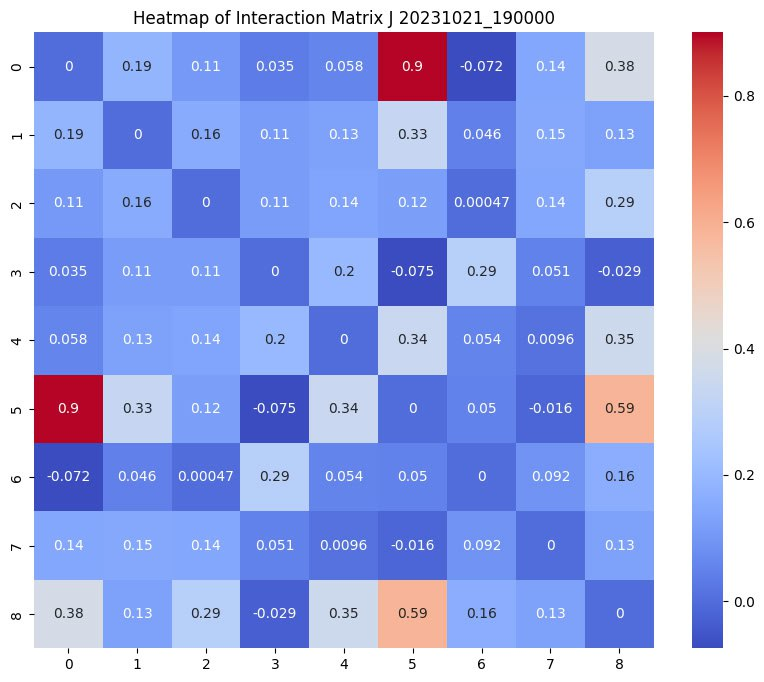
\includegraphics[width=\columnwidth]{assets/matrix_jij.jpg}
    \caption{Matriz de Interacciones \( J_{ij} \) Inferida para el 21 de octubre de 2023 a las 19:00 horas.}
    \label{fig:jij}
\end{figure}

Para facilitar la interpretación de las interacciones, se 
construye un grafo no dirigido donde cada nodo representa una 
rana y las aristas indican la presencia de una interacción 
inferida. En particular, se utiliza una línea continua para 
aquellas interacciones cuya magnitud supera el umbral de 0.5, 
y una línea discontinua para aquellas entre 0.3 y 0.5. 
Las interacciones por debajo de este último umbral se omiten 
por considerarse insignificantes. El resultado se muestra en la 
Figura~\ref{fig:graph}.

\begin{figure}[h!]
    \centering
    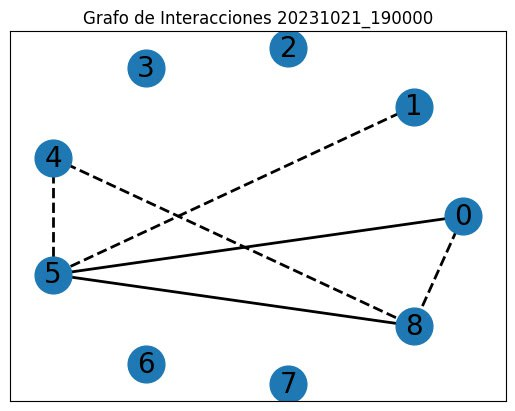
\includegraphics[width=\columnwidth]{assets/corr_graph.jpg}
    \caption{Grafo de Interacciones para el 21 de octubre de 2023 a las 19:00 horas.}
    \label{fig:graph}
\end{figure}

Como análisis preliminar, se aplicó el mismo procedimiento de 
inferencia a tres ventanas horarias consecutivas. 
En la Figura \ref{fig:jij_evol} se observa que algunas interacciones fuertes —particularmente 
aquellas por encima de 0.5— tienden a persistir en el tiempo, 
lo que sugiere la presencia de relaciones estables. 
Particularmente se nota que la interacción entre los índices 0 y 5 
perdura en las 3 horas en cuestión. En la Figura \ref{fig:graph_evol}
se visualiza como permanece la arista correspondiente en los respectivos grafos.
Este tipo de evidencia puede ser 
indicativo de organización funcional dentro del conjunto de 
ranas.

\begin{figure}[h!]
    \centering
    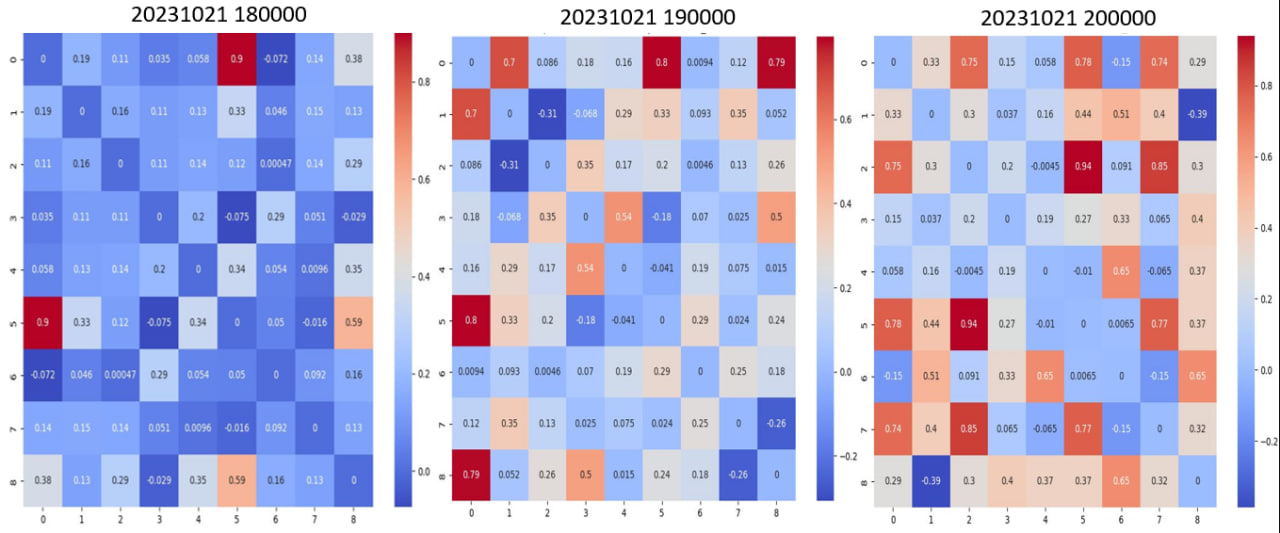
\includegraphics[width=\columnwidth]{assets/3_matrixs.jpg}
    \caption{Evolución de la matriz \( J_{ij} \) a lo largo de tres horas consecutivas.}
    \label{fig:jij_evol}
\end{figure}

\begin{figure}[h!]
    \centering
    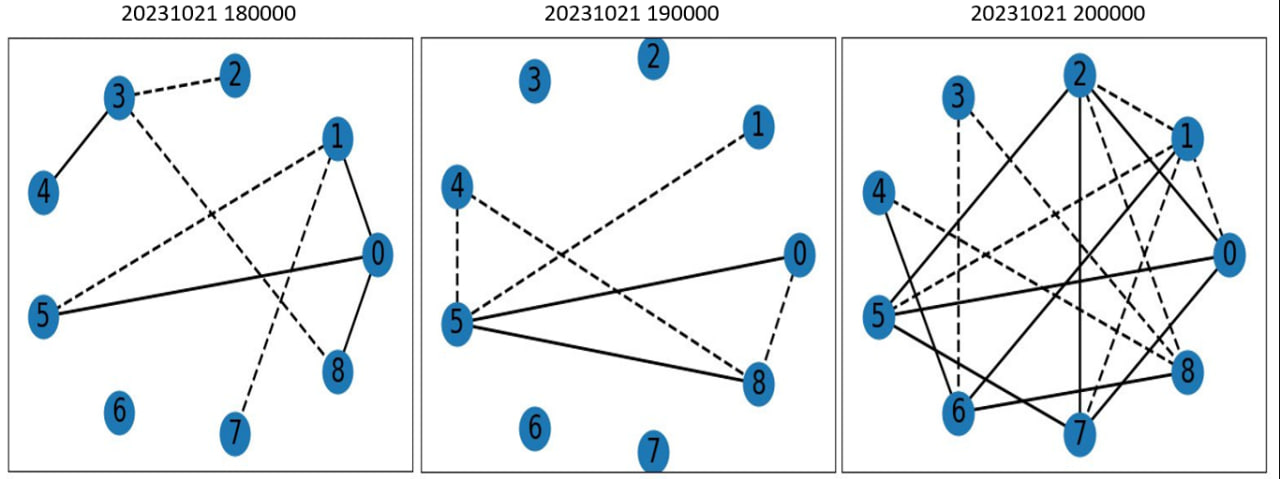
\includegraphics[width=\columnwidth]{assets/3_graphs.jpg}
    \caption{Evolución de los grafos de interacciones a lo largo de tres horas consecutivas.}
    \label{fig:graph_evol}
\end{figure}

%===================================================================================



%===================================================================================
% Conclusiones
%-----------------------------------------------------------------------------------
\section{Conclusiones}\label{sec:conc}

% El presente trabajo constituye una extensión significativa a 
% investigaciones anteriores en el análisis de coros de 
% \emph{Eleutherodactylus eileenae}. A partir de la 
% implementación de un algoritmo de inferencia basado en 
% descenso por gradiente y fundamentado en el Modelo de Ising, 
% se lograron identificar y cuantificar interacciones entre 
% individuos desde un enfoque basado en herramientas útiles, 
% principalmente
% de la Física Estadística. La capacidad de calcular 
% exactamente las expectativas del modelo, gracias al reducido 
% número de espines, permitió estimar los parámetros 
% \( J_{ij} \) y \( h_i \) sin recurrir a métodos de muestreo 
% estocástico, lo que se tradujo en resultados robustos y 
% reproducibles. Asimismo, las mejoras en la eliminación de ruido 
% y la sincronización automática de las grabaciones aportaron 
% mayor fidelidad a los datos, facilitando la detección de 
% relaciones fuertes y persistentes. Se concluye que la 
% aproximación propuesta es adecuada para descifrar la estructura 
% subyacente del comportamiento colectivo y sienta las bases para 
% análisis dinámicos y causales en sistemas biológicos complejos.

El presente trabajo constituye una extensión significativa a 
investigaciones anteriores en el análisis de coros de 
\emph{Eleutherodactylus eileenae}. A partir de la 
implementación de un algoritmo de inferencia basado en 
descenso por gradiente y fundamentado en el Modelo de Ising, 
se logró identificar y cuantificar las interacciones entre 
individuos desde un enfoque basado en herramientas de la Física 
Estadística. La capacidad de calcular exactamente las 
expectativas del modelo, dada la factibilidad de enumerar las 
\(2^9\) configuraciones posibles, permitió estimar los 
parámetros \( J_{ij} \) y \( h_i \) sin recurrir a métodos de 
muestreo estocástico, lo que se tradujo en resultados robustos 
y reproducibles. 

Particularmente, se observó que algunas interacciones 
muestran persistencia a lo largo de ventanas horarias 
consecutivas, lo que sugiere la existencia de una estructura 
definida y persistente en el comportamiento colectivo del coro. 
Esta persistencia indica que ciertos patrones de interacción, 
posiblemente relacionados con la organización funcional del 
grupo, se mantienen estables a lo largo del tiempo. 
Estos hallazgos no sólo confirman la robustez del enfoque 
propuesto, sino que también abren la puerta a futuros análisis 
dinámicos y causales en sistemas biológicos complejos, 
especialmente en contextos en los que el sistema opera fuera 
del equilibrio termodinámico, tal como ocurre en la realidad.

%===================================================================================



%===================================================================================
% Recomendaciones
%-----------------------------------------------------------------------------------
\section{Recomendaciones}\label{sec:rec}

Se recomienda continuar investigando la dinámica temporal de las interacciones, explorando métodos alternativos y enfoques que permitan analizar la causalidad de los cantos en condiciones de desequilibrio termodinámico. Asimismo, es pertinente profundizar en la hipótesis planteada en el trabajo anterior acerca de la posible regulación voluntaria de la frecuencia en los cantos, la cual podría ser un mecanismo para distinguir a los individuos dentro del coro. La exploración de estos aspectos contribuirá a una comprensión más integral de la organización y el comportamiento colectivo en sistemas biológicos acústicos.



%===================================================================================



%===================================================================================
% Bibliografía
%-----------------------------------------------------------------------------------
% \begin{thebibliography}{99}
% %-----------------------------------------------------------------------------------
% 	\bibitem{knuth} Donald E. Knuth. \emph{The Art of Computer Programming}.
% 		Volume 1: Fundamental Algorithms (3rd~edition), 1997.
% 		Addison-Wesley Professional.

% 	\bibitem{goedel} Kurt Göedel. \emph{Über formal unentscheidbare Sätze der
% 		Principia Mathematica und verwandter Systeme, I}.
% 		Monatshefte für Mathematik und Physik 38.

% 	\bibitem{wiki} Wikipedia. URL: \href{http://en.wikipedia.org}
% 	  {http://en.wikipedia.org}.
% 		Consultado en \today.

% %-----------------------------------------------------------------------------------
% \end{thebibliography}

% \bibliographystyle{babplain}
\bibliography{build/sample}


%-----------------------------------------------------------------------------------

\label{end}

\end{document}

%===================================================================================
